\chapter{Evaluation}

\section{Introduction}

\begin{itemize}
    \item Talk about why the three sections below are being talked about
\end{itemize}


\section{Interconnect Performance}

Calling a function implemented in hardware off-chip is not latency free. There will be some overhead latency associated with packaging the data to be sent over the channel, sending the data over the channel itself, and then repeating this process in order to return the data produced by the off-chip function back to the main FPGA. Therefore, it is of importance to measure this overhead so that we can gauge the efficiency of the interconnect hardware that was designed for SystemNaim.

Since the decision was made to implement an SPI communication channel for the final product, we had to into consideration the SPI clock speed used by the system. On an SPI channel, a single bit is sent on every cycle of the SPI clock meaning it takes 32 SPI Clock cycles to send single 32-bit integer. Increasing the SPI Clock speed allows for a higher performing channel, which is able to send data in a shorter period, however, this increase comes at the cost of reliability. This section explores the effect of the SPI Clock rate on a test system. We will attempt to prove that increasing the clock speed does reduce the total overhead, but will also investigate the overhead added from the interconnect to the latency of the system.

\subsection{Test Model}

In order to find out how much of the latency of a multi-FPGA system, created in SystemNaim, can be attributed to the interconnect, we must first devise a model that can tell us what data needs to be gathered. At it's most simple, we can model the latency of a system as the sum of the time taken to perform the actual processing i.e. the code that the user entered into the tool, and the time taken to encode, transmit, receive, and decode the data across the SPI channel i.e. the overhead. \autoref{eqn:tot_sys_latency}, shows the mathematical equivalent of the previous statement.

\begin{equation}
    L_{sys} = L_{processing} + L_{overhead}
    \label{eqn:tot_sys_latency}
\end{equation}

In order to find $L_{processing}$ from \autoref{eqn:tot_sys_latency} we make the following assumption: the total processing time, in cycles, for a multi-FPGA system is the same as a single FPGA system where both the off-chip function and on-chip function, from the former system, are run in parallel. In essence, if we measure the latency of a system that has been created on a single FGPA using SystemNaim's “split” keyword then we can assume the total latency of this system is equal to $L_{processing}$ for a multi-FPGA system where “split” has been replaced with “split-fpga”.

Before we continue an important side note, $L_{rest}$ will refer to the latency caused by the processing outside the function call i.e. the processing before and after the function call. In terms of hardware SystemNaim generates the exact same in both the single FPGA and multi-FPGA case before and after the function call. Furthermore, for simplicity the single FPGA system with parallel hardware will be called the Multi-Thread Single Chip (MTSC) system, as it denotes parallel computation on a single chip, likewise, the multi-FPGA system will be referred to as the Multi-Thread Multi-Chip (MTMC) system. 

We can prove that $L_{processing} = L_{MTSC}$, where $L_{MTSC}$ is the total latency for an MTSC system, if we place the following constraint on the system: all parallel functions in the system must have the same latency.

\autoref{fig:multi_func_call} is a diagram representing the program path for a multi-function call in an MTSC system. As can be seen the total latency $L_f = max(L_1,L_2)$, however with our constraint $L_1 = L_2$, and thus we can simplify to \autoref{eqn:fcl_2}. \autoref{fig:multi_fpga_call} shows a similar diagram for the MTMC case. Assuming both functions are the same and that $L_{I1} > 0 \&\& L_{I2} > 0 $ then equations \ref{eqn:mtmc_latency_start} to \ref{eqn:mtmc_latency} hold. 

\begin{align}
    &L_{f\_MTSC} = L_1 \label{eqn:fcl_1} \\
    &L_{MTSC} = L_{rest} + L_1 \label{eqn:fcl_2}
\end{align}

\begin{align}
    &L_{f\_MTMC} = max(L_1 + L_{I1} + L_{I2} , L_2) = L_1 + L_{I1} + L_{I2} \label{eqn:mtmc_latency_start} \\
    &L_{MTMC} = L_{rest} + L_1 + L_{I1} + L_{I2}  \\
    &L_{MTMC} = L_{MTSC} + L_{I1} + L_{I2} \\
    \therefore \; &L_{processing} = L_{MTSC} \label{eqn:mtsc_processing} \\
    \& \; &L_{overhead} = L_{I1} + L_{I2} 
    \label{eqn:mtmc_latency}
\end{align}

Given those results we prove that we can use the MTSC latency in the MTMC calculations. We also proved that the overhead was $L_{overhead} = L_{I1} + L_{I2}$, which represents the latency incurred by sending and receiving data over the channel and seems like a sensible representation of the overhead. Furthermore, \autoref{eqn:overhead_formula} show's that we can calculate the overhead latency by finding the difference between the latency of an MTMC and MTSC system, provided that they both call the same functions and have the same processing before and after the function call. In SystemNaim this is easily doable by switching the “split” keyword with “split-fpga”. 

\begin{align}
    &L_{MTMC} = L_{processing} + L_{overhead} \\
    &L_{overhead} = L_{MTMC} - L_{processing}  \\
    &L_{overhead} = L_{MTMC} - L_{MTSC}\label{eqn:overhead_formula}
\end{align}

\begin{figure}[!htb]
    \centering
    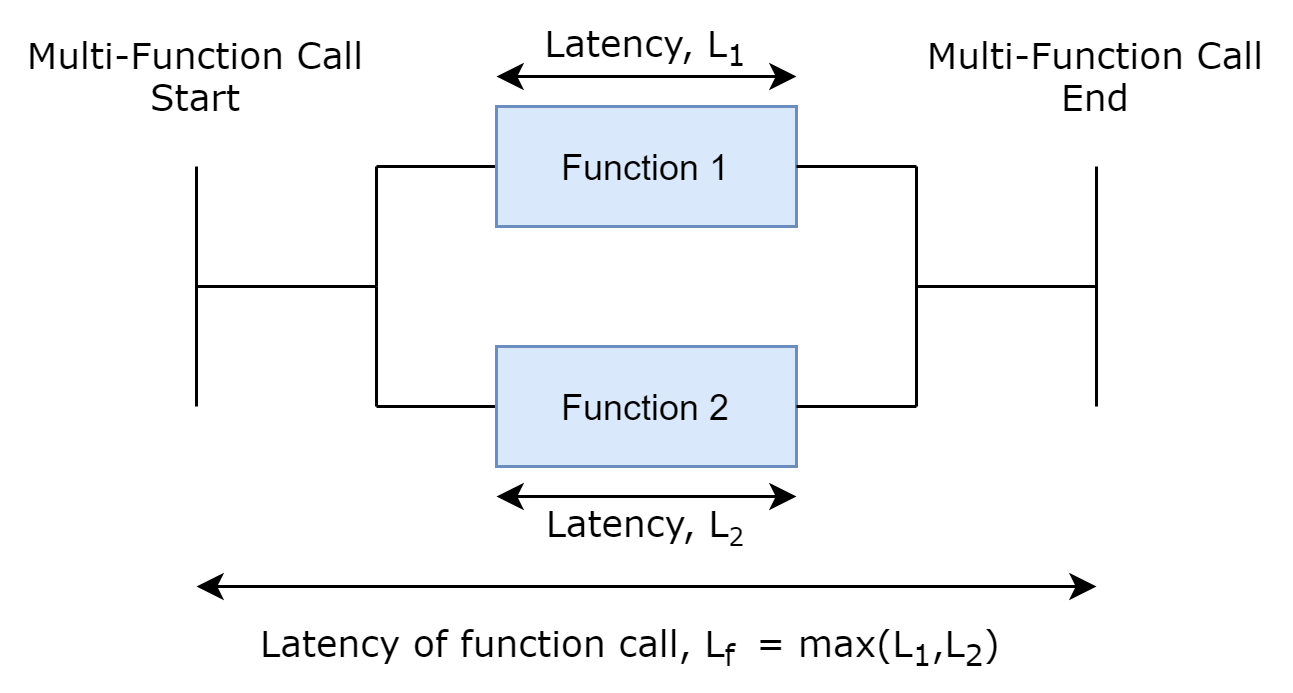
\includegraphics[width=0.9\textwidth]{05_evaluation/images/concurrent_latency.png}
    \caption{Latency of single FPGA multi-function call}
    \label{fig:multi_func_call}
\end{figure}

\begin{figure}[!htb]
    \centering
    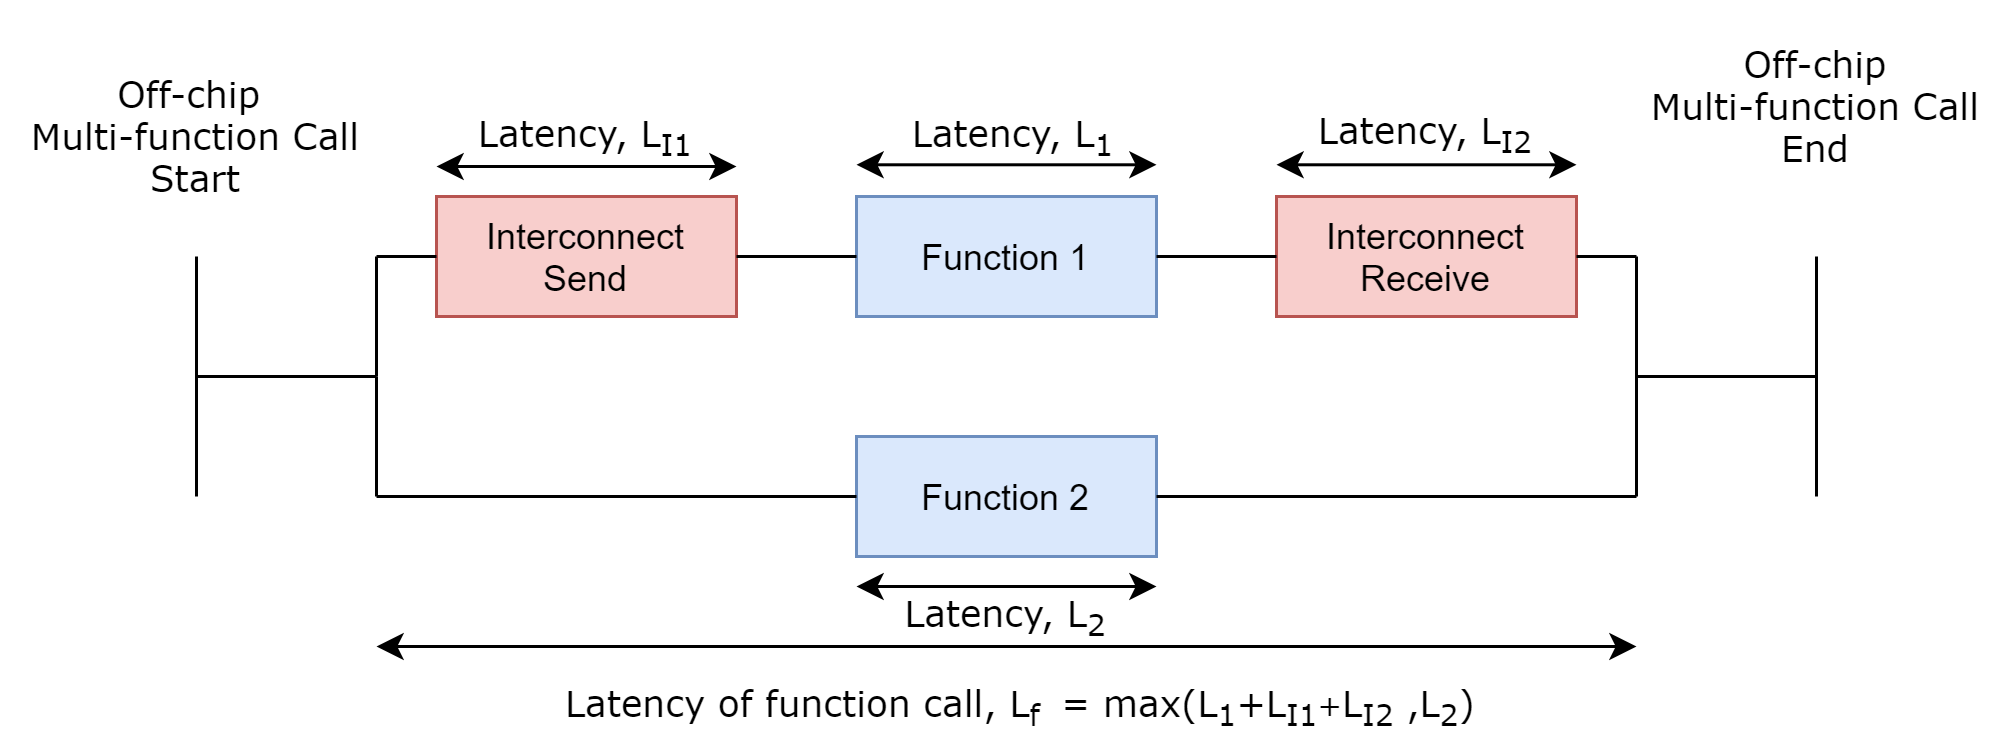
\includegraphics[width=0.9\textwidth]{05_evaluation/images/offchip_latency.png}
    \caption{Latency of multi FPGA multi-function call}
    \label{fig:multi_fpga_call}
\end{figure}

\subsection{Channel Bandwidth}
 
We can further dissect the overhead latency and split it into two parts. The transfer overhead, $L_{t\_overhead}$, which is latency cost incurred for transmitting and receiving data over a channel and the interconnect overhead, $L_{i\_overhead}$, which is the latency cost from encoding and decoding the data transmitted. Essentially, the latter part comes from the hardware designed specifically for SystemNaim, whereas the former is merely the limit of the channel. In an ideal world the interconnect overhead would be 0 and only the transfer overhead would exist. 

We can calculate the transfer overhead by knowing the rate at which data is transferred over the channel, and in the case of an SPI channel this is dependent on the SPI clock speed, $\mathit{SPI}_{clock}$. The SPI clock speed is different from the system clock speed, $\mathit{SYS}_{clock}$; both can be configured by the user but in our case we have a variable SPI clock speed and a static system clock speed at 50MHz.

Our SPI channel transfers data at 1 bit per SPI clock cycle, which is standard, however we're not interested in how long it takes for data to be transferred relative to the SPI clock. Instead, we would like to know how many system clock cycles it takes to transmit a single bit. We'll refer to this value as the channel latency, $L_{channel}$, and it can be calculated by dividing the system clock speed by the SPI clock speed. The resulting value has a unit of cycles per bit.

For SystemNaim, we know that any off-chip function call requires 128 bits of data to be sent over the channel. 96 bits (or 3 integers) are required to send the opcode, operand A and operand B, while the last 32 bits are for the data that needs to be returned to the main FPGA. Therefore, the formula for the transfer overhead, which is measure of how many clock cycles it takes to transfer all the data over a channel for an off-chip function call, is shown in \autoref{eqn:overhead}. 

\begin{equation}
    L_{channel} = \frac{\mathit{SYS}_{clock}}{\mathit{SPI}_{clock}} 
    \label{eqn:clock_speed}
\end{equation}

\begin{equation}
    L_{t\_overhead} = 128 * L_{channel}
    \label{eqn:overhead}
\end{equation}

\subsection{Testing}

With the maths and the modelling in place we can now being testing the system to see if we can get an experimental value for the overhead and how it is affected by the SPI clock speed. For this test we use a program which calls 2 function, which are syntactically the same, and then exits. We first compile the program with both functions being called within a “split” block and test the latency of this MTSC system. Afterwards we test the same program, but we replace the “split” keyword with the “split-fpga” keyword, this will be the MTMC system. 

The MTMC system will be run multiple times with varying SPI clock speeds, and for each test we will compare the latencies between the MTMC and MTSC systems, compute the transfer overhead and find the interconnect overhead.

\subsection{Results}

\autoref{tbl:spi_clk_results} shows the data gathered, in accordance to testing methodology laid out above. It should be noted that the \textbf{Channel Latency} and \textbf{Est. Transfer Overhead} columns have been calculated using no gathered data. Both columns are dependent on the \textbf{SPI Clock (Hz)}, and the calculations for each can be found in Equation \ref{eqn:clock_speed} and \ref{eqn:overhead} respectively.

\autoref{fig:spi_clk_graph} is a summation of the important data from the table in the form of graph, thus making it easier to identify trends in the data.

\begin{sidewaystable}
    \centering
    \begin{threeparttable}
    \begin{tabular}{l|l|l|l|l|l}
    \textbf{SPI Clock (Hz)} & \textbf{Channel Latency} & \textbf{Latency (Cycles)} & \textbf{Overhead (Cycles)} & \textbf{Transfer Overhead} & \textbf{Interconnect Overhead} \\ \hline
     125,000               &  400                 &  52,918              &  52,794              & 51,200                &  1,594                                      \\
     250,000               &  200                 &  26,518              &  26,394              & 25,600                &  794                                        \\
     252,525\tnote{*}      &  198                 &  26,254              &  26,130              & 25,344                &  786                                        \\
     277,777\tnote{*}      &  180                 &  23,878              &  23,754              & 23,040                &  714                                        \\
     312,500               &  160                 &  26,532              &  26,408              & 20,480                &  5,928                                      \\
     347,222\tnote{*}      &  144                 &  23,892              &  23,768              & 18,432                &  5,336                                      \\
     500,000               &  100                 &  16,632              &  16,508              & 12,800                &  3,708                                      \\
     1,000,000             &  50                  &  8,382               &  8,258               & 6,400                 &  1,858                                      \\
     1,923,076\tnote{*}    &  26                  &  4,422               &  4,298               & 3,328                 &  970                                        \\
     5,000,000             &  10                  &  1,782               &  1,558               & 1,280                 &  278                                        \\
     8,333,333\tnote{*}    &  6                   &  1,122               &  998                 & 768                   &  230                                        \\
     12,500,000            &  4                   &  792                 &  668                 & 512                   &  156                                        \\
     25,000,000            &  2                   &  542                 &  418                 & 256                   &  162                                       
    \end{tabular}
    \begin{tablenotes}\footnotesize
        \item[*] These values for SPI clock speed are not factors of the system clock, and are actually irrational.
        \end{tablenotes}
    \end{threeparttable}
    \caption{Effect of SPI clock speeds on overhead latency}
    \label{tbl:spi_clk_results}
\end{sidewaystable}

\begin{figure}[!htb]
    \centering
    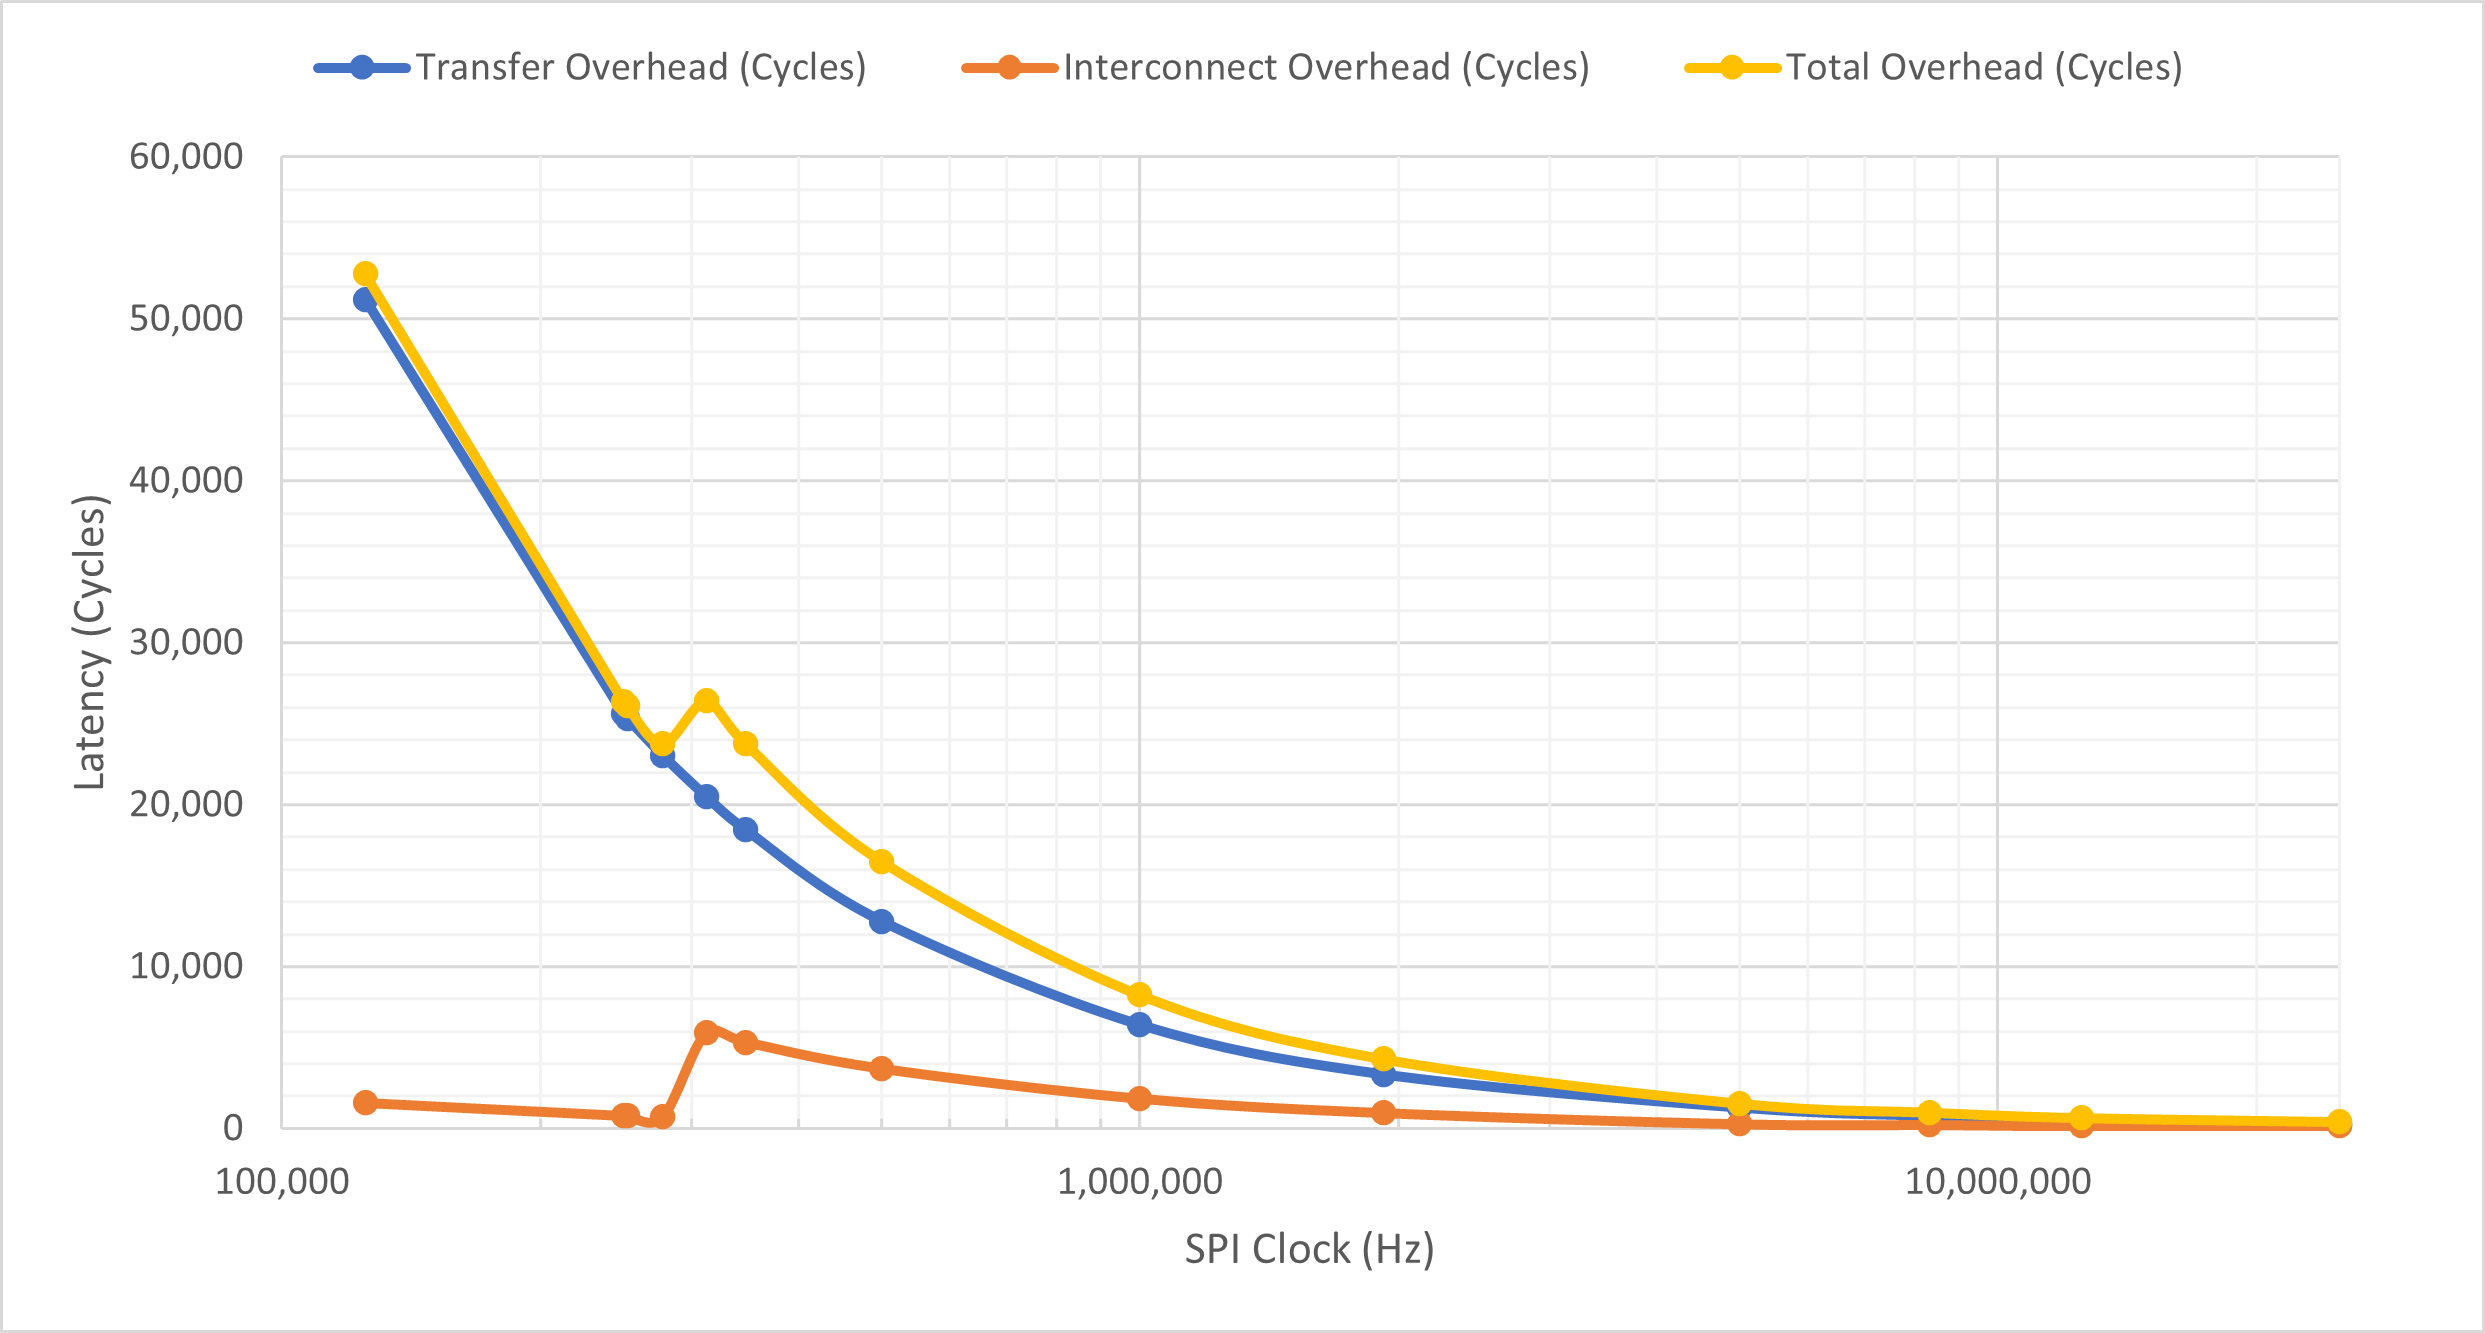
\includegraphics[width=0.9\textwidth]{05_evaluation/images/overhead_vs_spi_clk.png}
    \caption{Overhead Latency vs. SPI Clock Speed \textit{(Best case would be that the total overhead equals the transfer overhead)}} 
    \label{fig:spi_clk_graph}
\end{figure}


\subsection{Conclusions}

Generally speaking, we can conclude that as we increase the SPI clock speed the total overhead latency decreases, we can also deduce that the main proportion of the overhead is transfer overhead. This is supported by \autoref{fig:spi_clk_graph}, and was the result we intended for this investigation to prove. However, there are a few interesting caveats to this conclusion that we cannot ignore. Firstly, while not shown on the graph or table, during testing it was found that setting the clock speed the values higher than 8MHz resulted in increased channel instability. Tests would occasionally fail to complete with transactions not being detected by either the on-chip or off-chip interconnect, the higher the clock speed the more likely this phenomenon would occur.

This instability may have been caused by the physical components of the channel not being able to accurately keep up with these speeds. For the final product GPIO pins on both FPGAs were connected using breadboard jumper cables, which aren't intended to be used for data communication. Potentially, at clock speeds of 8MHz and above, the GPIO pins were not able to go from high to low, and vice versa, fast enough to generate a detectable clock on the child FPGA. The fault could also lie with the SPI core and the FPGA hardware. The SPI core takes in the main system clock, generates the SPI Clock and transmits that signal to a GPIO pin. Therefore, there may be an issue between the pin and the FPGA hardware. Unfortunately, there's no way to be certain of the cause, and instead we can only conclude that speeds above 8MHz result in unreliable performance. 

The more interesting result from the gathered data, however, comes from the trend of the \textbf{Interconnect Overhead}. While it would be expected that the latency from the interconnect would be generally static, with only minor fluctuations since the task of encoding data should be uniform, what we see instead is a generally decreasing trend except for a steep rise in latency at 312,500Hz. This behaviour, however, makes complete sense given the design of the interconnect and is a consequence of the SPI channel only allowing the master to initiate transactions. 

As explained in SOME IMPLEMENTATION SECTION, the child FPGA cannot indicate to the parent FPGA when it has completed processing its off-chip function. Therefore, in order to receive the return data the parent FPGA must continuously send polling transactions on the SPI channel. When any transaction is started by the master SPI core on the parent FPGA, the slave SPI core starts simultaneously transmitting data stored in an internal register. At some point during operation, this internal register will contain the result of the off-chip function call, but that point cannot be determined beforehand and thus arises the need for continuous polling transactions, a diagram of this process is shown in \autoref{fig:interconnect_polling}. Because of this, when the off-chip function is complete, and it passes the result to the SPI slave core, the core must wait for the current polling transaction to finish before the next one starts, and then it can send the valid return data. Therein lies the issue, the wait for a current transaction to finish.

The worst case for this scenario is if the slave SPI core has to wait for a full transaction, minus one cycle, to complete before it can send its data. At lower clock rates this can take thousands of cycles, more specifically $32 * L_channel$ cycles, since each transaction consists of 32 bits. Furthermore, how close the end time of an off-chip function is to the end of any given polling transaction is dependent on both the SPI clock speed and the latency of the function itself, therefore it becomes incredibly difficult to avoid the worse case scenario and the interconnect overhead becomes stochastic in nature. However, we can minimize the interconnect overhead by increasing the SPI clock speed, as this reduces the number of system cycles it takes for a polling transaction to finish and thus also the number of system cycles the slave SPI core has to wait in the worse case scenario.

In conclusion, we should try to maximize the SPI clock speed as this reduces the transfer overhead, and minimizes the worst case for the interconnect overhead, thus, increasing the performance of the MTMC system.


\begin{figure}[!htb]
    \centering
    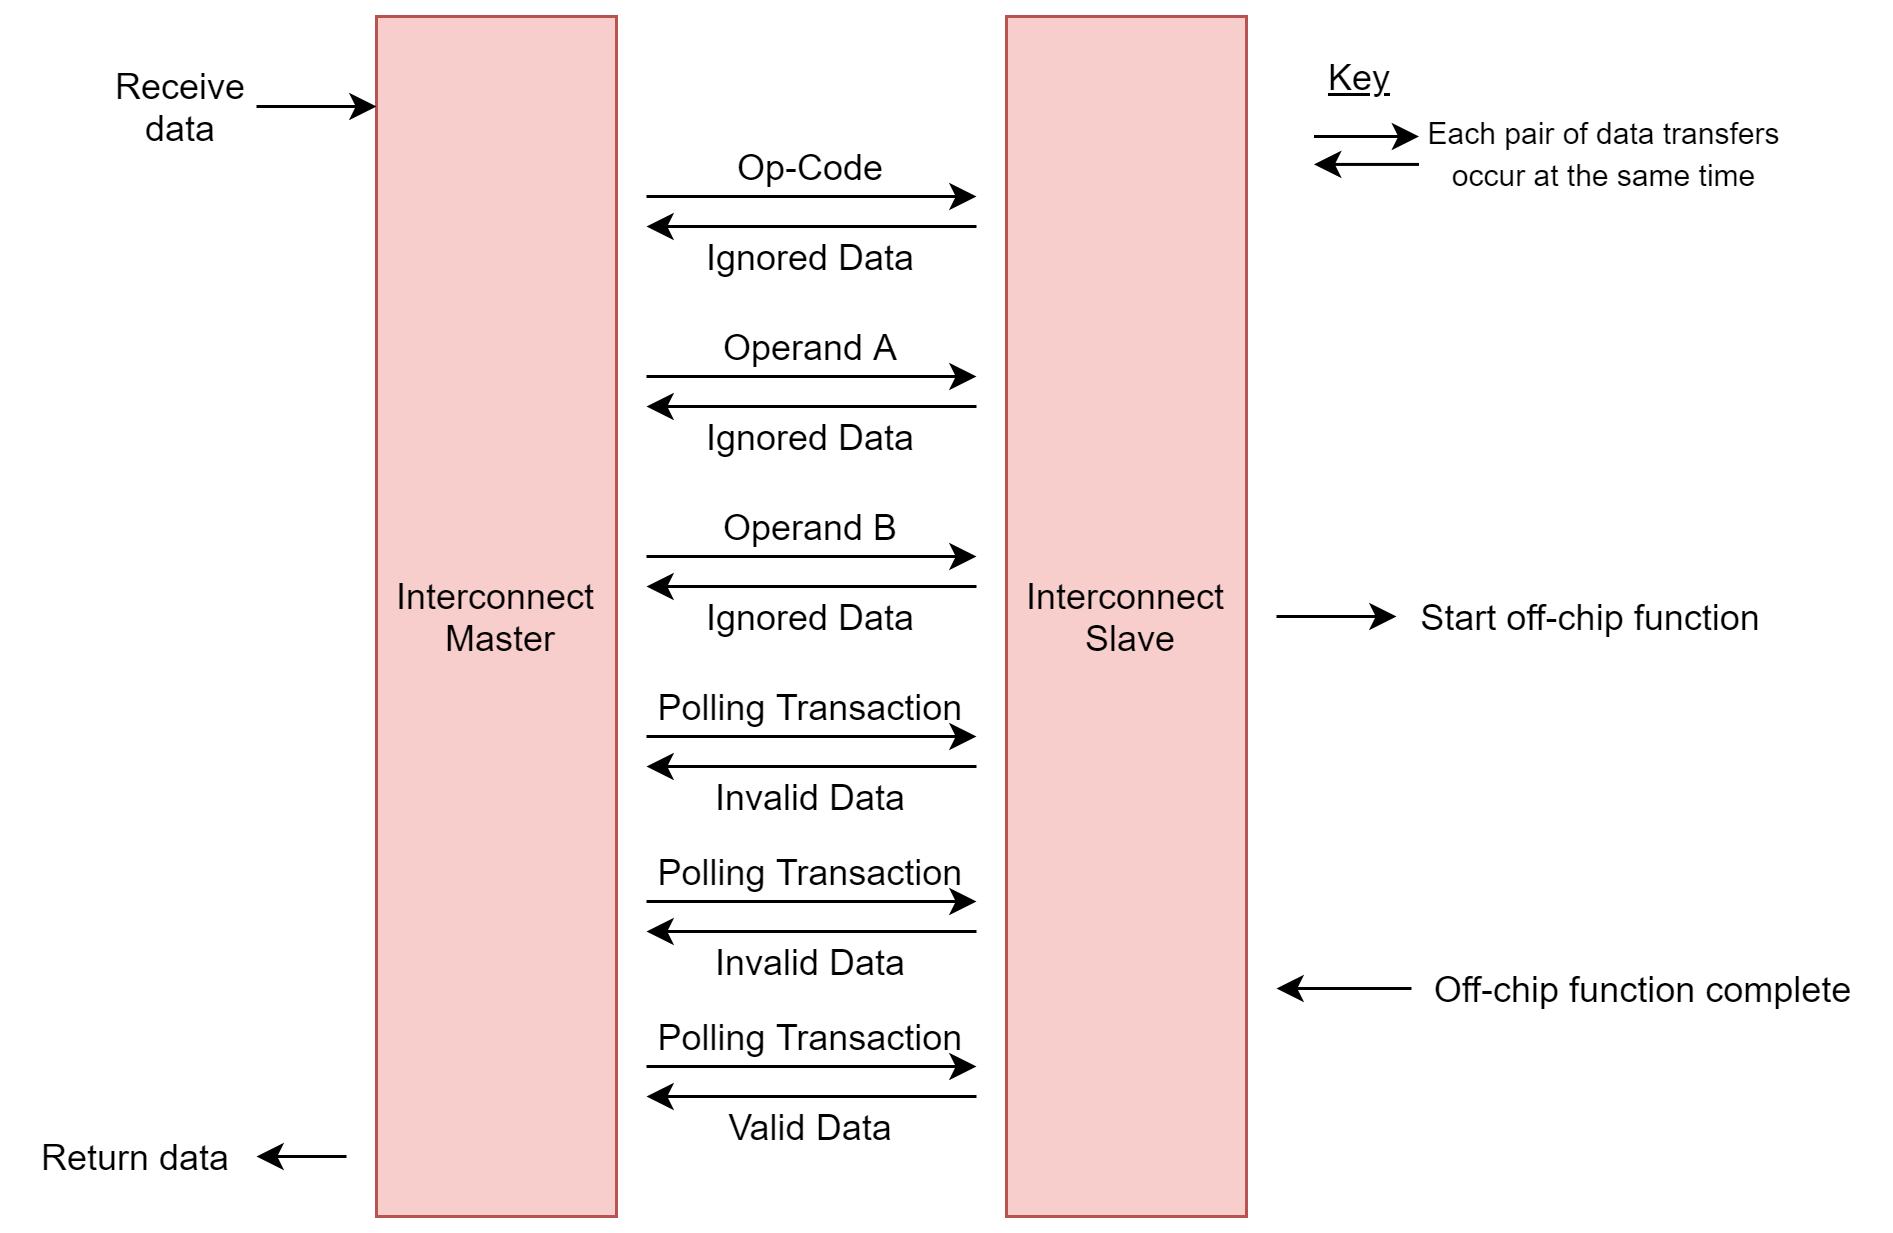
\includegraphics[width=0.9\textwidth]{05_evaluation/images/interconnect_polling.png}
    \caption{Example of interconnect communication protocol in practice}
    \label{fig:interconnect_polling}
\end{figure}


\section{System Performance}
\label{sec:sys_perf}

Now that we have established that higher SPI clock speeds, and also higher channel bandwidths, reduce the total overhead associated with calling a function off-chip, we can start to explore what kind of programs can exploit the benefits of a multi-FPGA system the best. In general, FPGAs are mainly used for their ability to exploit parallelism in programs, and the motivation for using multiple FPGAs in tandem is to access more resources (LUTs, BRAM, DSPs etc.). Therefore, it stands to reason that the best programs to run on a multi-FPGA system are one which can have large parts of the processing run in parallel but also require a large amount of resources.

Considering the limitations of SystemNaim it would be difficult for us to write programs which take up a large percentage of an FPGAs resources, however, we can investigate how well we can exploit a program's affinity for parallelism and how the same program performs on a single FPGA system versus a multi-FPGA system. Ideally, we will be able to prove that as program latency increases the percentage contribution of the interconnect overhead to the total latency will decrease, thus, giving more credence to using a multi-FPGA system.

\subsection{Test Model}

The model for this investigation is relatively straightforward. We will write a numerical integration program and using SystemNaim, run the program on three different systems. The first will be a full sequential program with no parallelism, the second will exploit the parallelism of the program, but all processing will happen on a single FPGA, the final system will be a multi-FPGA one, which will also exploit the parallelism of the program but will also perform some processing on a second FPGA.

Borrowing from the previous investigation each system will have a short-hand to make them easier to identify. The sequential system will be the Single-Thread Single Chip (STSC) system, the single FPGA system with parallelism will be the Multi-Thread Single Chip (MTSC) system and finally the multi-FPGA system will be the Multi-Thread Multi-Chip (MTMC) system.

The program that we will be running will contain loops that run for a fixed number of iterations. As we vary the number iterations, we will measure the latency of each system at each step and compare the results. Furthermore, we will dissect the MTMC latency into processing latency and overhead, where the overhead is a measure of the cost incurred, in cycles, for perform part of the processing off-chip.

As a final note, the SPI core in this investigation will be set at 5MHz or 10\% of the system clock. This decision was made in order minimize channel latency, while maintaining reliability.

\subsection{Numerical Integration Program}

The numerical integration method that we decided to implement was the Composite Simpson's rule, which is shown in \autoref{eqn:comp_simp}. What makes this specific implementation interesting to us are the two sums, $s_1$ and $s_2$. These sums can be easily setup so that they are computed in parallel when implemented in SystemNaim. All that is needed is to make functions of each sum and call them within a “split” or “split-fpga” block to produce either an MTSC or MTMC system respectively. $n$, is also chosen by the user, and we can increase that to increase the number of total iterations the program must make.

Unfortunately, since a function in SystemNaim can only have two numerical inputs there are some limitations on the program. The first is that $a$, the lower bound of the integral will be a compile-time constant, thus, unmodifiable during runtime. The second is that both functions will have knowledge of what $f(x)$ is at runtime, and will make calls to a function in software which computes the value of $f(x)$. Each of these calls in software will create a module in hardware, resulting in two hardware modules which compute $f(x)$. This, however, is necessary for the parallelism and will allow for some interesting analysis that will be explored later on.

The final issue is unrelated to the two input problem, but is due to SystemNaim not supporting floats. Only integers are supported and to ensure we produce valid results, care has been taken in order to choose $a$, $b$, $n$, and $h$ such that no decimal values are produced during operation.

Overall, none of the three issues disrupt the purpose of the investigation at hand, which focuses on how the latency of the systems are affected as we increase the number iterations the program has to run. However, in the interest of a fair and open investigation it was deemed important to include them.

\begin{align}
    & s_1(f(x),n,a,h) = 2 \sum_{j=1}^{n/2-1}f(x_{2j}) \text{, where } x_j = a + jh \\
    & s_2(f(x),n,a,h) = 4 \sum_{j=1}^{n/2}f(x_{2j-1}) \text{, where } x_j = a + jh \\
    &\int_{a}^{b} f(x) dx \approx \frac{h}{3} \Big[ f(x_a) + s_1(f(x),n,a,h) + s_2(f(x),n,a,h) + f(x_b) \Big] \text{, where } h = \frac{b-a}{n}  \label{eqn:comp_simp}
\end{align}

\subsection{Results}

\autoref{tbl:system_results} shows the results of the investigation. \autoref{fig:latency_v_iter} shows the same data but in the form of graph in order to be able to identify trends more easily.
Finally, \autoref{fig:overhead_percent} shows the percentage contribution of the overhead to the MTMC latency, however, this graph needs a slight amount of justification before we can draw conclusions from it.

The investigation has been designed in such a manner that the MTSC and MTMC systems are exploiting the same amount of parallelism in the program and are preforming the same amount of processing. The only difference is that the MTMC must also go through the trouble of calling a function off-chip, which has been proved to incur a latency cost. Therefore, we assume that the processing latency i.e. the amount of cycles spent executing the code that the user entered into the tool, are the same for both systems. Thus, the difference between the two latencies is the cost incurred to call a function off-chip and is therefore the latency. This was much more rigorously proved in the previous investigation but the reasoning above provides an adequate platform for this section.

Finally, by comparing the MTSC latency and the calculate overhead we can guage what percentage of the total latency of the MTMC system was due to the off-chip function call and thus evaluate whether the jump from single FPGA to multi-FPGA is worth the latency cost. 

\begin{sidewaystable}
    \centering
    \begin{tabular}{l|l|l|l|l|l}
    \textbf{Iterations ($n$)} & \textbf{STSC Latency (Cycles)} & \textbf{MTSC Latency (Cycles)} & \textbf{MTMC Latency (Cycles)} & \textbf{Overhead (Cycles)}\\ \hline
     200        & 2,572               & 1,370                 & 2,839                 &  1,469                 \\
     400        & 5,072               & 2,670                 & 4,215                 &  1,545                 \\
     600        & 7,572               & 3,970                 & 5,591                 &  1,621                 \\
     800        & 10,072              & 5,270                 & 6,967                 &  1,697                 \\
     1000       & 12,572              & 6,570                 & 7,999                 &  1,429                 \\
     1200       & 15,072              & 7,870                 & 9,375                 &  1,505                 \\
     1400       & 17,572              & 9,170                 & 10,751                &  1,581                 \\
     1600       & 20,054              & 10,470                & 12,127                &  1,657                 \\
     1800       & 22,572              & 11,770                & 13,503                &  1,733                 \\
     2000       & 25,072              & 13,070                & 14,535                &  1,465                 \\                                 
    \end{tabular}
    \caption{Effect of Program iterations on total latency}
    \label{tbl:system_results}
\end{sidewaystable}

\begin{figure}[!htb]
    \centering
    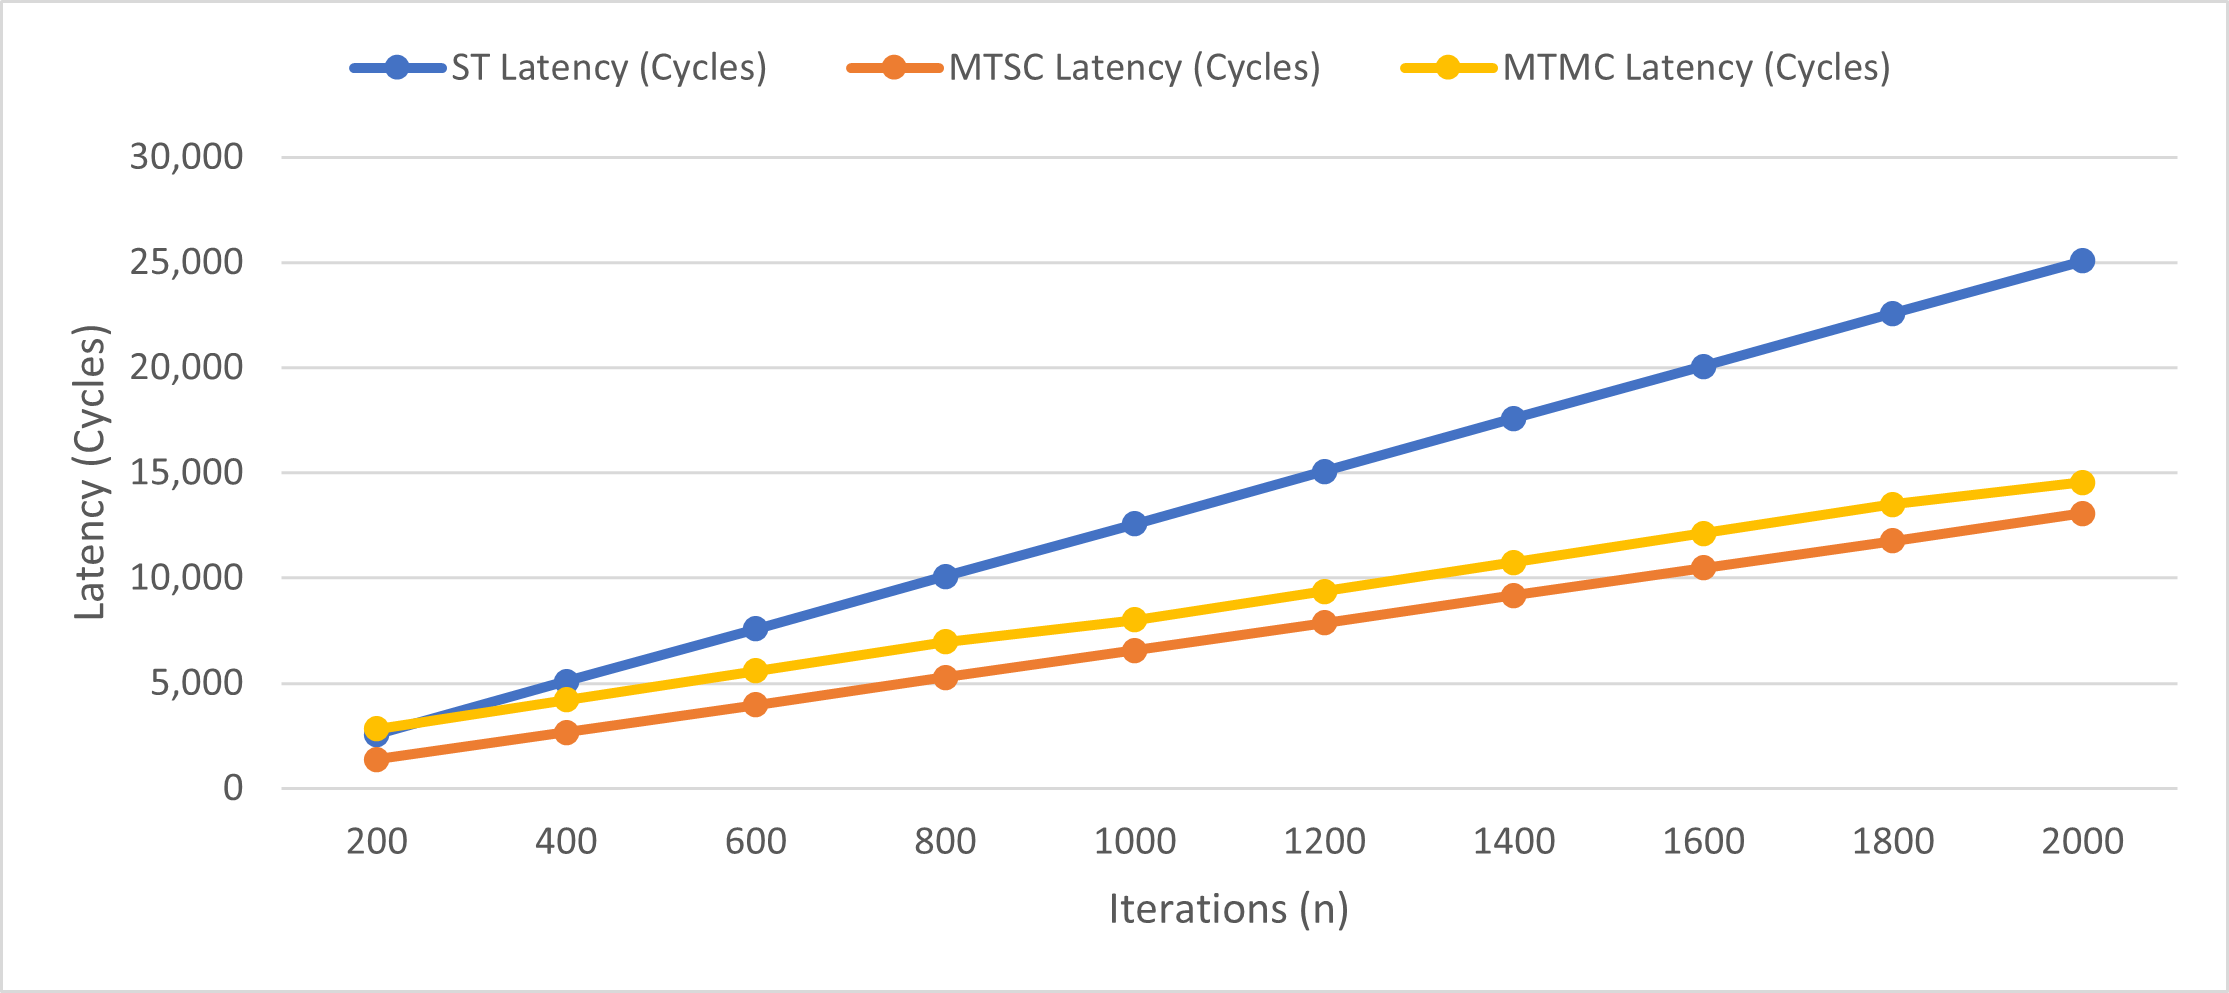
\includegraphics[width=0.9\textwidth]{05_evaluation/images/latency_vs_iter.png}
    \caption{Latencies of different systems as iterations of program increase}
    \label{fig:latency_v_iter}
\end{figure}

\begin{figure}[!htb]
    \centering
    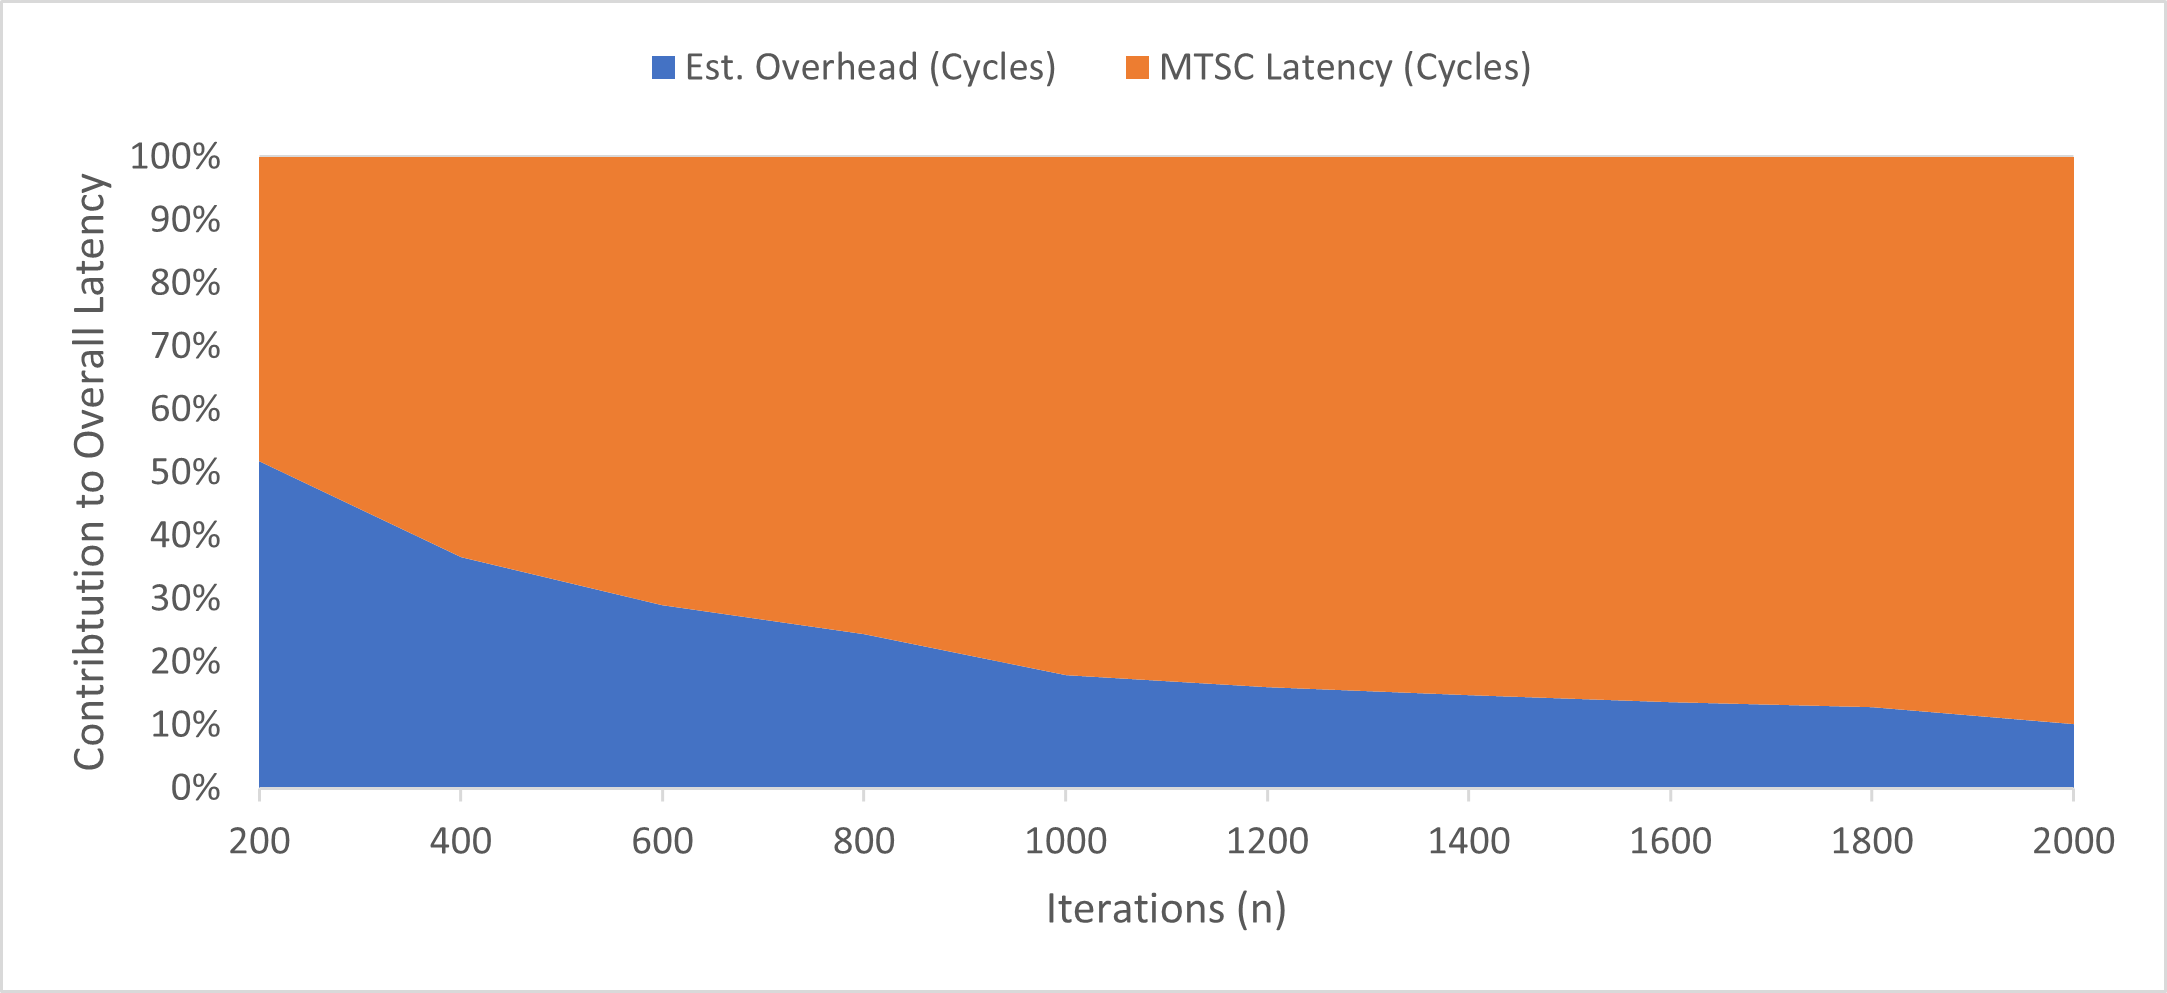
\includegraphics[width=0.9\textwidth]{05_evaluation/images/overhead_percentage.png}
    \caption{Percentage contribution of overhead to total latency}
    \label{fig:overhead_percent}
\end{figure}

\subsection{Conclusions}

Our main conclusion from this investigation is that as we increase the number of iterations the program has to perform the overhead in the MTMC system contributes less to the overall latency. This claim is supported by \autoref{fig:overhead_percent}, as you can see that with a declining trend in the percentage contribution from the overhead as iterations increases. What we can then conclude is that MTMC systems in which the off-chip function has a large processing latency will perform more equally to their MTSC equivalent systems, therefore, it advised to users of SystemNaim to code their programs in such a way that the designated off-chip function has as much processing time as possible i.e. it has a loop with a large bound within it. One thing of note, is that the stochastic nature of the interconnect is likely due to the polling issue mentioned in the previous investigation, however as can be seen in \autoref{tbl:system_results}, the overhead tends to be centred around an average value of 1,570 cycles which is close to the overhead measured in \autoref{tbl:spi_clk_results} for the 5MHz SPI clock, the same speed as the SPI clock in this investigation. The range of the measured overheads is 304 cycles, thus, the total overhead latency will be at most 20\% away from the average. This can be seen as an issue for programs with low latencies, but as mentioned above those programs wouldn't be advisable for SystemNaim.

Further, by observing the relationship between the latency of the STSC and MTSC system in \autoref{fig:latency_v_iter}, and \autoref{tbl:system_results}, we can see that exploiting the parallelism in the program gave us approximately a 2x speed up, this is due to the fact that there were two sums, $s_1$ and $s_2$, that we calculated in parallel. We can extrapolate from this and say that if you had a program which had three segments which could be run in parallel you would be able to achieve a 3x speed up, and as you increase the number of parallel segments, be they a loop or some other part of the program, you can achieve further performance increases. Therefore, it is advisable to users of SystemNaim to analyse, and potentially rewrite, to exploit as much parallelism as possible.

However, a user must be careful in where they place their off-chip function call. If placed within a loop the overhead does not occur once, but rather it occurs for every iteration. Now this may not be too much of a concern if the processing latency of the off-chip function hardware is high relative to the overhead, but it would be preferable to try and reduce the number of calls to off-chip functions to reduce the contribution the overhead latency makes to the total latency of the system.

One final thing that can be discussed is the necessity for the both the MTSC and MTMC systems to instantiate two hardware modules to calculate $f(x)$. While not the case in this investigation, the hardware module for $f(x)$ may potentially be very resource intensive, specifically, mathematical functions tend to use a lot of DSPs. In the case where a single FPGA may not have enough DSPs to instantiate two modules to compute $f(x)$, you would no longer be able to create an MTSC system. As an example if each $f(x)$ module took 3 DSPs and our FPGA only had $5$, we would be one short of the required $6$. The user's options would then either be to run the system sequentially, and achieve the results of an STSC system, or it would be to instead use multi-FPGA solution and utilize an MTMC system. This would be a real-world motivation for using a multi-FPGA system, in order to get a latency reduction, and thus provides credence to the purpose of SystemNaim.



\section{Usability}

\begin{itemize}
    \item This section is a qualitative analysis on how difficult the tool is to use. 
    \item Since there's not enough time to ask others to evaluate the tool, a comparison will be made between using the tool to make a multi-FPGA system, and starting from scratch just implementing hardware in Verilog. While it won't be completely accurate, it should be somewhat realistic as I can take inspiration from how long it took me to create certain aspects such as the interconnect.
    \item Make sure to mention that in a pure hardware implementation you probably wouldn't create a giant state machine like the tool generations, instead you'd create a very focused piece of hardware.
\end{itemize}

One of the major motivations of SystemNaim is increasing the accessibility of multi-FPGA systems to people who may not be very hardware proficient. The way we have tried to tackle this goal is by creating a HLS tool which requires knowledge of C90 and basic programming constructs, therefore allowing the tool to be used by a larger group. 

In order to illustrate the usability of the tool we will go through a design example and then perform a qualitative comparison to creating the same system but purely in Quartus II using only SystemVerilog and the IP catalogue.

\subsection{Design Example: Numerical Integration}

For this design example we have decided to show how we implemented the Composite Simpson numerical integration method that was used in the investigation in \autoref{sec:sys_perf}.

The first step for any user would be to write the C code. For this example in particular this took around 15 minutes and the original 
